\documentclass[a4paper,11pt]{article}
\usepackage[utf8]{inputenc}
\usepackage[T1]{fontenc}
\usepackage[a4paper,top=1in, bottom=1in, left=1in, right=1in]{geometry}
\usepackage[french,magyar]{babel}
\def\magyarOptions{defaults=prettiest}

\usepackage[none]{hyphenat}
\usepackage{amsfonts,amsmath,amssymb}
\usepackage{fancyhdr}
\usepackage[none]{hyphenat}

\usepackage{hyperref}
\hypersetup{
    colorlinks=true,
    linkcolor=black,
    filecolor=magenta,      
    urlcolor=blue,
}

\usepackage[nottoc,notlot,notlof]{tocbibind}
\usepackage{graphicx}
\usepackage{caption}
\usepackage{subfig}
\usepackage{enumitem}
\usepackage{booktabs}
\usepackage[export]{adjustbox}
\usepackage{enumitem}
\setlist[1]{itemsep=-5pt}
\pagestyle{fancy}
\fancyhead{}
%\fancyfoot{}
\renewcommand{\headrulewidth}{0pt}

\usepackage{hyperref}

\usepackage{listings}
 
\urlstyle{same}

%\renewcommand{\baselinestretch}{1.5}

\begin{document}
%\emergencystretch 3em
\sloppy

\begin{titlepage}
\begin{center}
%\vspace{1cm}
\begin{figure}[t!]
	\begin{center}
	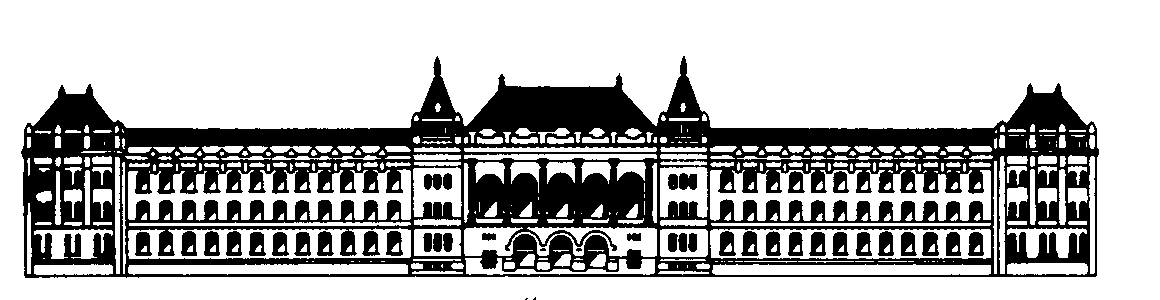
\includegraphics[scale=0.2]{bme.png}
	\label{a:bme}
	\end{center}
\end{figure}
\textbf{{Budapesti Műszaki és Gazdaságtudományi Egyetem}}\\
Villamosmérnöki és Informatikai Kar\\
Méréstechnika és Információs Rendszerek Tanszék\\
\vfill
\huge\textbf{{Rendszerarchitektúrák}}\\[3mm]
\Large{Házi feladat}\\[3mm]
\Large\textbf{{AXI - SPI perifériaillesztő}}\\
\vfill
\Large{Kardos Bálint, ZI84PX}\\
\Large{Murányi Péter, A74MW9}\\
\Large{Konzulens: Raikovich Tamás}\\
\vfill
\today \\

\end{center}
\end{titlepage}

\tableofcontents
\thispagestyle{empty}
\clearpage

\setcounter{page}{1}
\setcounter{tocdepth}{4}
\setcounter{secnumdepth}{4}
\setlength{\parindent}{2em}
%\setlength{\parskip}{1em}

\section{}


\section{}

\subsection{}

\subsection{}

\subsection{}

\subsubsection{}

\subsubsection{}


\section{SPI modul működése}

\subsection{}

\subsection{}


\section{Szimuláció}
A létrehozott periféria működése szimulációval lett ellenőrizve. A szimulációhoz a Vivado beépített szimulátorát használtuk. A perifériához az AXI interfész felől egy AXI-LITE Master-t szimuláló BFM lett illesztve, míg az SPI oldalról egy Microchip EEPROM funkcionális verilog modellje lett illesztve. A szimuláció egy az EEPROM-ba való írást, majd onnan a beírt adatok kiolvasását valósítja meg.

A szimuláció 100MHz-s órajelet használ, a reset vonal induláskor 20ns ideig aktív alacsony állapotban van, majd visszatér magas szintre, ami elindítja az összes eszközt.

Az SPI modul /16 órejelosztást használ, amivel az SCK 6,25 MHz lesz.
\subsection{BFM}

\subsection{EEPROM}
Az eszközhöz egy Microchip 25AA010A EEPROM szimulációs verilog modellje van illesztve, hogy a valós működés is tesztelve legyen. Ez a modul egy 1kbit méretű flash EEPROM-ot valósít meg, valós időzítési értékekkel. Az eszköz leírása \href{http://ww1.microchip.com/downloads/en/DeviceDoc/21832H.pdf}{ezen a linken} érhető el.

Az eszköz valós időzítéseket is szimulál, ezért például az SCK órajel nem lehet gyorsabb 10MHz-nél, ugyanis az eszköz nem lesz képes elég gyorsan reagálni az órajel változására. Ezt az SPI órajelosztójának megfelelő beállításával lehet elérni.

Hogy az eszközt írhassuk, először egy instrukciót kell neki küldeni ami engedélyezi az írást az eszközön belül. Ehhez egy külön írási ciklusra van szükségünk ahol $\overline{CS}$ jelet aktív alacsonyra kell húzni, majd az írásengedélyező (WREN) parancsot kiküldve a $\overline{CS}$ jelet egy órajelciklus idejére vissza kell engedni magas szintre. Ha ezt nem tesszük meg, nem fogunk tudni írni az eszközbe. Ezek után lehet ténylegesen írni az eszközt. Íráskor először egy 8-bites írás instrukciót kell kiküldeni, ez után jöhet a cím, szintén 8-biten, majd ezt követően kezdődik meg a tényleges adat kiküldése. Lehet bájtos, illetve burst módban írni, viszont burst módban maximum 16 bájtot lehet kiküldeni, ugyanis az EEPROM csak ekkora bemeneti bufferrel rendelkezik. Az írást a $\overline{CS}$ magasra húzásával lehet befejezni, ekkor az írásengedélyező belső flag automatikusan 0-ra áll vissza. Az EEPROM verilog modelljében apró változtatásokat kellett eszközölni, ugyanis a valóságot szimulálva 5ms-ig késleltet mielőtt az adatot ténylegesen beírja az adattároló regisztereibe. Ezt hogy a szimuláció rövidebb legyen, és a kapott hullámformák átláthatóbbak legyenek 100ns-re csökkentettük.

\subsection{Szimuláció eredménye}


\section{Forráskód}

\subsection{SPI és busz illesztő}

\subsubsection{}

\subsubsection{}

\subsection{}

\subsubsection{}

\subsection{}

\subsubsection{}


\section{}


\pagebreak
\begin{thebibliography}{}

\bibitem{name1}

\textit{}
\url{  }
\today

\bibitem{name2}

\textit{}\\
\url{}
\today

\bibitem{name3}

\textit{}\\
\url{}
\today

\bibitem{name4}

\textit{}\\
\url{}
\today

\bibitem{name5}

\textit{}\\


\bibitem{name6}

\textit{}\\
\url{}
\today


\end{thebibliography}
\end{document}
